\documentclass[11pt,a4paper]{article}
\usepackage[T1]{fontenc}
\usepackage[utf8]{inputenc}
\usepackage{lmodern}
\usepackage[margin=22mm]{geometry}
\usepackage{amsmath,booktabs,longtable,graphicx}
\usepackage{xcolor,listings,textcomp}
\usepackage[hidelinks]{hyperref}
\hypersetup{pdftitle={Tutorial 1: LV Voltage Estimation - Exercise Solutions},pdfauthor={},pdfsubject={Exercise Solutions}}
\definecolor{codeblue}{RGB}{29,72,117}
\definecolor{codegreen}{RGB}{40,105,68}
\definecolor{codebackground}{RGB}{247,248,250}
\lstset{
  language=Python,
  basicstyle=\ttfamily\footnotesize,
  keywordstyle=\color{codeblue}\bfseries,
  commentstyle=\color{codegreen},
  stringstyle=\color{codeblue},
  backgroundcolor=\color{codebackground},
  frame=single,rulecolor=\color{black!15},
  breaklines=true,breakatwhitespace=false,
  columns=fullflexible,keepspaces=true,
  showstringspaces=false,upquote=true,tabsize=4,
  xleftmargin=4pt,xrightmargin=4pt,
  aboveskip=10pt,belowskip=10pt
}
\setlength{\parindent}{0pt}
\setlength{\parskip}{6pt}
\title{Tutorial 1: LV Voltage Estimation\\Exercise Solutions}
\author{}
\date{}

\begin{document}
\maketitle

\section*{Before running the solutions}
These solutions cover all seven tasks in Tutorial 1. In a fresh
notebook kernel, run Sections 2.2--2.4 of
\path{Tutorial_1_LV_Voltage_Estimation.ipynb} first. Then paste
the Python listings into the matching Exercise Workspace cells and run
them in order. The main tutorial search in Sections 2.5--2.6 does not need
to be repeated.

The listings reuse the notebook's data and helper functions. The model
has 62 P/Q inputs and 31 voltage outputs; there are no Vref inputs in
Tutorial 1. All power and voltage data are simulated. This is same-time
voltage estimation, not forecasting.

Each exercise fit uses 40 epochs, batch size 72, learning rate $10^{-3}$
and L2 strength $10^{-5}$. The exercise budget is independent of the
tutorial's quick/full mode. Scalers must be fitted on training rows only.
Select the configuration and seed using training-data folds; do not use
the test set until E2.3. The exercise reuses the tutorial's test period for
a classroom comparison, not a new independent evaluation.

\section*{E1.1: 93 hidden neurons with tanh}
Evaluate the starting configuration on three consecutive validation
blocks. The helper trains a fresh model for each block and returns
fold errors in volts. Store a copy of the configuration with its scores
so later changes do not alter this result.

\begin{lstlisting}[title={E1.1}]
e1_config = {
    "hidden_neurons": 93,
    "activation": "tanh",
    "lr": 1e-3,
    "weight_decay": 1e-5,
    "batch_size": 72,
    "epochs": 40,
}
e1_seed = 42
e1_k = 3
e1_rows = []
e1_scores = evaluate_config(
    e1_config, PQ_tr, V_tr, k=e1_k, seed=e1_seed
)
e1_row = e1_config.copy()
e1_row.update(e1_scores)
e1_rows.append(e1_row)
print(
    f"E1.1: RMSE = {e1_scores['RMSE_kfold']:.6f} V; "
    f"std = {e1_scores['RMSE_std']:.6f} V"
)
\end{lstlisting}

\section*{E1.2: Increase the hidden-neuron count to 155}
Change only the hidden-neuron count. Keep the activation, other training
settings, seed and validation folds unchanged.

\begin{lstlisting}[title={E1.2}]
e1_config_155 = e1_config.copy()
e1_config_155["hidden_neurons"] = 155
e1_scores_155 = evaluate_config(
    e1_config_155, PQ_tr, V_tr, k=e1_k, seed=e1_seed
)
e1_row_155 = e1_config_155.copy()
e1_row_155.update(e1_scores_155)
e1_rows.append(e1_row_155)
print(
    f"E1.2: RMSE = {e1_scores_155['RMSE_kfold']:.6f} V; "
    f"std = {e1_scores_155['RMSE_std']:.6f} V"
)
\end{lstlisting}

\section*{E1.3: Add the ReLU cases and select a configuration}
Add the two ReLU cases to the two stored tanh results; do not retrain the
earlier cases just to display the comparison. Four cases and three folds
require $4\times3=12$ fits. Select using unrounded mean validation RMSE.
The standard deviation is the population standard deviation of the three
fold scores (\texttt{ddof=0}), not a confidence interval.

\begin{lstlisting}[title={E1.3}]
for e1_neurons in [93, 155]:
    e1_relu_config = e1_config.copy()
    e1_relu_config["hidden_neurons"] = e1_neurons
    e1_relu_config["activation"] = "relu"
    e1_relu_scores = evaluate_config(
        e1_relu_config, PQ_tr, V_tr, k=e1_k, seed=e1_seed
    )
    e1_relu_row = e1_relu_config.copy()
    e1_relu_row.update(e1_relu_scores)
    e1_rows.append(e1_relu_row)

e1_results = pd.DataFrame(e1_rows).sort_values(
    "RMSE_kfold", kind="stable"
).reset_index(drop=True)
assert len(e1_results) == 4
display(e1_results[[
    "hidden_neurons", "activation", "epochs",
    "RMSE_kfold", "RMSE_std",
]].round(6))

e1_best_row = e1_results.iloc[0]
e1_best_config = {
    "hidden_neurons": int(e1_best_row["hidden_neurons"]),
    "activation": str(e1_best_row["activation"]),
    "lr": float(e1_best_row["lr"]),
    "weight_decay": float(e1_best_row["weight_decay"]),
    "batch_size": int(e1_best_row["batch_size"]),
    "epochs": int(e1_best_row["epochs"]),
}
print("Selected configuration:", e1_best_config)

# Store exercise results separately from the tutorial.
e1_results_directory = (
    TUTORIAL_DIRECTORY / "results" / "exercises"
)
e1_results_directory.mkdir(parents=True, exist_ok=True)
e1_results.to_csv(
    e1_results_directory / "exercise_configurations.csv",
    index=False,
)
\end{lstlisting}

\section*{E2.1: Compare seeds 0, 1 and 2}
Keep \texttt{e1\_best\_config} unchanged. Use the same three training-data
folds for each seed. This comparison requires $3\times3=9$ fresh fits.

\begin{lstlisting}[title={E2.1}]
e2_seeds = [0, 1, 2]
e2_seed_results = run_seed_search(
    PQ_tr, V_tr, e1_best_config, e2_seeds, k=e1_k
)
e2_seed_results = e2_seed_results.sort_values(
    "RMSE_kfold", kind="stable"
).reset_index(drop=True)
display(e2_seed_results[[
    "seed", "RMSE_kfold", "RMSE_std"
]].round(6))
e2_selected_seed = int(e2_seed_results.iloc[0]["seed"])
print("Configuration:", e1_best_config)
print("Selected seed:", e2_selected_seed)
e2_seed_results.to_csv(
    e1_results_directory / "exercise_seeds.csv",
    index=False,
)
\end{lstlisting}

\section*{E2.2: Train a new model on all training rows}
Fit new input and target scalers on all training data. Build a fresh
model, not a fold model or the tutorial's final model. This last fit
brings the exercise total to $12+9+1=22$ fits.

\begin{lstlisting}[title={E2.2}]
e2_input_scaler = MinMaxScaler().fit(PQ_tr)
e2_output_scaler = MinMaxScaler().fit(V_tr)
e2_X_train = e2_input_scaler.transform(
    PQ_tr
).astype(np.float32)
e2_Y_train = e2_output_scaler.transform(
    V_tr
).astype(np.float32)

e2_model = build_model(
    2 * C, C, e1_best_config, seed=e2_selected_seed
)
e2_history = train_model(
    e2_model, e2_X_train, e2_Y_train, e1_best_config
)
e2_model.summary()
print("Completed epochs:", len(e2_history.epoch))
assert len(e2_history.epoch) == 40
assert e2_model.input_shape[-1] == 62
assert e2_model.output_shape[-1] == 31

import json
e2_settings = {
    "configuration": e1_best_config,
    "selected_seed": e2_selected_seed,
    "folds": e1_k,
    "training_fits": 22,
    "completed_epochs": len(e2_history.epoch),
    "network_parameters": int(e2_model.count_params()),
}
with (e1_results_directory / "exercise_settings.json").open(
    "w", encoding="utf-8"
) as settings_file:
    json.dump(e2_settings, settings_file, indent=2)
\end{lstlisting}

\section*{E2.3: Estimate test voltages and calculate errors}
Use \texttt{transform()}, not \texttt{fit()} or
\texttt{fit\_transform()}, on test inputs. Convert predictions back to
volts before evaluating them. For $N$ time steps and $C=31$ customers,
\[
\mathrm{RMSE}=\sqrt{\frac{1}{NC}\sum_{t=1}^{N}\sum_{c=1}^{C}
(\widehat V_{t,c}-V_{t,c})^2},\qquad
\mathrm{MAE}=\frac{1}{NC}\sum_{t=1}^{N}\sum_{c=1}^{C}
|\widehat V_{t,c}-V_{t,c}|.
\]
For per-customer RMSE, average squared errors over time only.

\begin{lstlisting}[title={E2.3}]
e2_X_test = e2_input_scaler.transform(
    PQ_te
).astype(np.float32)
e2_V_estimated = predict_unscaled(
    e2_model, e2_X_test, e2_output_scaler
)
assert e2_V_estimated.shape == V_te.shape == (2016, 31)
assert np.isfinite(e2_V_estimated).all()
e2_error = e2_V_estimated - V_te
e2_rmse = float(np.sqrt(np.mean(e2_error ** 2)))
e2_mae = float(np.mean(np.abs(e2_error)))
e2_customer_rmse = np.sqrt(np.mean(e2_error ** 2, axis=0))

e2_metrics = pd.DataFrame({
    "Metric": ["RMSE", "MAE"],
    "Value (V)": [e2_rmse, e2_mae],
})
e2_customer_errors = pd.DataFrame({
    "Customer": np.arange(1, C + 1),
    "RMSE (V)": e2_customer_rmse,
})
display(e2_metrics.round(6))
display(e2_customer_errors.round(6))
e2_metrics.to_csv(
    e1_results_directory / "exercise_test_metrics.csv",
    index=False,
)
e2_customer_errors.to_csv(
    e1_results_directory / "exercise_customer_rmse.csv",
    index=False,
)
\end{lstlisting}

\section*{E2.4: Inspect the highest-RMSE customer}
The array position is zero-based; add one to display the customer number.
Inspect this customer after evaluation without retuning the model.
Residuals are estimated voltage minus simulated reference voltage.

\begin{lstlisting}[title={E2.4}]
e2_worst_customer = int(np.argmax(e2_customer_rmse))
print(
    f"Customer {e2_worst_customer + 1}: "
    f"RMSE = {e2_customer_rmse[e2_worst_customer]:.6f} V"
)
e2_hours = np.arange(len(V_te)) * MINUTES_PER_STEP / 60
e2_fig, e2_axes = plt.subplots(
    2, 1, figsize=(11, 6), sharex=True
)
e2_axes[0].plot(
    e2_hours, V_te[:, e2_worst_customer],
    color="black", label="Simulated reference",
)
e2_axes[0].plot(
    e2_hours, e2_V_estimated[:, e2_worst_customer],
    color="tab:blue", label="Estimated", alpha=0.8,
)
e2_axes[0].set_ylabel("Voltage (V)")
e2_axes[0].set_title(
    f"Exercise 2: Customer {e2_worst_customer + 1}"
)
e2_axes[0].legend()
e2_axes[1].plot(
    e2_hours, e2_error[:, e2_worst_customer],
    color="tab:red", linewidth=0.8,
)
e2_axes[1].axhline(0, color="black", linestyle="--")
e2_axes[1].set_xlabel("Hours from start of test period")
e2_axes[1].set_ylabel("Estimate - reference (V)")
e2_axes[1].set_title("Voltage residual")
e2_fig.tight_layout()
e2_fig.savefig(
    e1_results_directory / "exercise_worst_customer.png",
    dpi=160, bbox_inches="tight",
)
plt.show()
\end{lstlisting}

\section*{Verified execution example}
These results are from an actual execution of the seven listings above.
The code selects settings from unrounded validation scores; the recorded
values are an example, not constants to hard-code into model selection.
Numerical results may vary slightly across environments.

All 22 exercise fits completed on CPU. The test set contains 2,016 rows and 31 customers.

\subsection*{E1.1--E1.3: Configuration comparison}

\begin{center}
\begin{tabular}{rlrrr}
\toprule
Hidden neurons & Activation & Epochs & Mean RMSE (V) & Std. (V) \\
\midrule
155 & tanh & 40 & 0.075256 & 0.003544 \\
93 & tanh & 40 & 0.081666 & 0.004465 \\
155 & relu & 40 & 0.088692 & 0.003253 \\
93 & relu & 40 & 0.103469 & 0.008829 \\
\bottomrule
\end{tabular}
\end{center}

Selected configuration: 155 hidden neurons, tanh, learning rate $10^{-3}$, L2 strength $10^{-5}$, batch size 72 and 40 epochs.

\subsection*{E2.1: Seed comparison}

\begin{center}
\begin{tabular}{rrr}
\toprule
Seed & Mean validation RMSE (V) & Std. (V) \\
\midrule
1 & 0.069666 & 0.003863 \\
0 & 0.075048 & 0.002759 \\
2 & 0.076155 & 0.002292 \\
\bottomrule
\end{tabular}
\end{center}

Selected seed: 1.

\subsection*{E2.2: Final network}

The final model has 62 inputs, 31 outputs and 14,601 network parameters. It completed 40 epochs on all 6,048 training rows. Keras may also show optimizer-state parameters in its summary; these are not additional neurons or trainable network weights.

\subsection*{E2.3: Held-out test errors}

\begin{center}
\begin{tabular}{lr}
\toprule
Metric & Value (V) \\
\midrule
RMSE & 0.054894 \\
MAE & 0.039941 \\
\bottomrule
\end{tabular}
\end{center}

\begin{longtable}{rr}
\caption{Test RMSE for every target customer.}\\
\toprule Customer & RMSE (V) \\ \midrule
\endfirsthead
\toprule Customer & RMSE (V) \\ \midrule
\endhead
\bottomrule\endfoot
1 & 0.038563 \\
2 & 0.039443 \\
3 & 0.041992 \\
4 & 0.041317 \\
5 & 0.040860 \\
6 & 0.038897 \\
7 & 0.045386 \\
8 & 0.041216 \\
9 & 0.051875 \\
10 & 0.046413 \\
11 & 0.052481 \\
12 & 0.048988 \\
13 & 0.069180 \\
14 & 0.032063 \\
15 & 0.040150 \\
16 & 0.045766 \\
17 & 0.077979 \\
18 & 0.085399 \\
19 & 0.073828 \\
20 & 0.054317 \\
21 & 0.076296 \\
22 & 0.059683 \\
23 & 0.067354 \\
24 & 0.039922 \\
25 & 0.053868 \\
26 & 0.075472 \\
27 & 0.055716 \\
28 & 0.042674 \\
29 & 0.058709 \\
30 & 0.048059 \\
31 & 0.062222 \\
\end{longtable}

\subsection*{E2.4: Highest-RMSE customer}

Customer 18 has the highest test RMSE: 0.085399 V.

\begin{figure}[htbp]
  \centering
  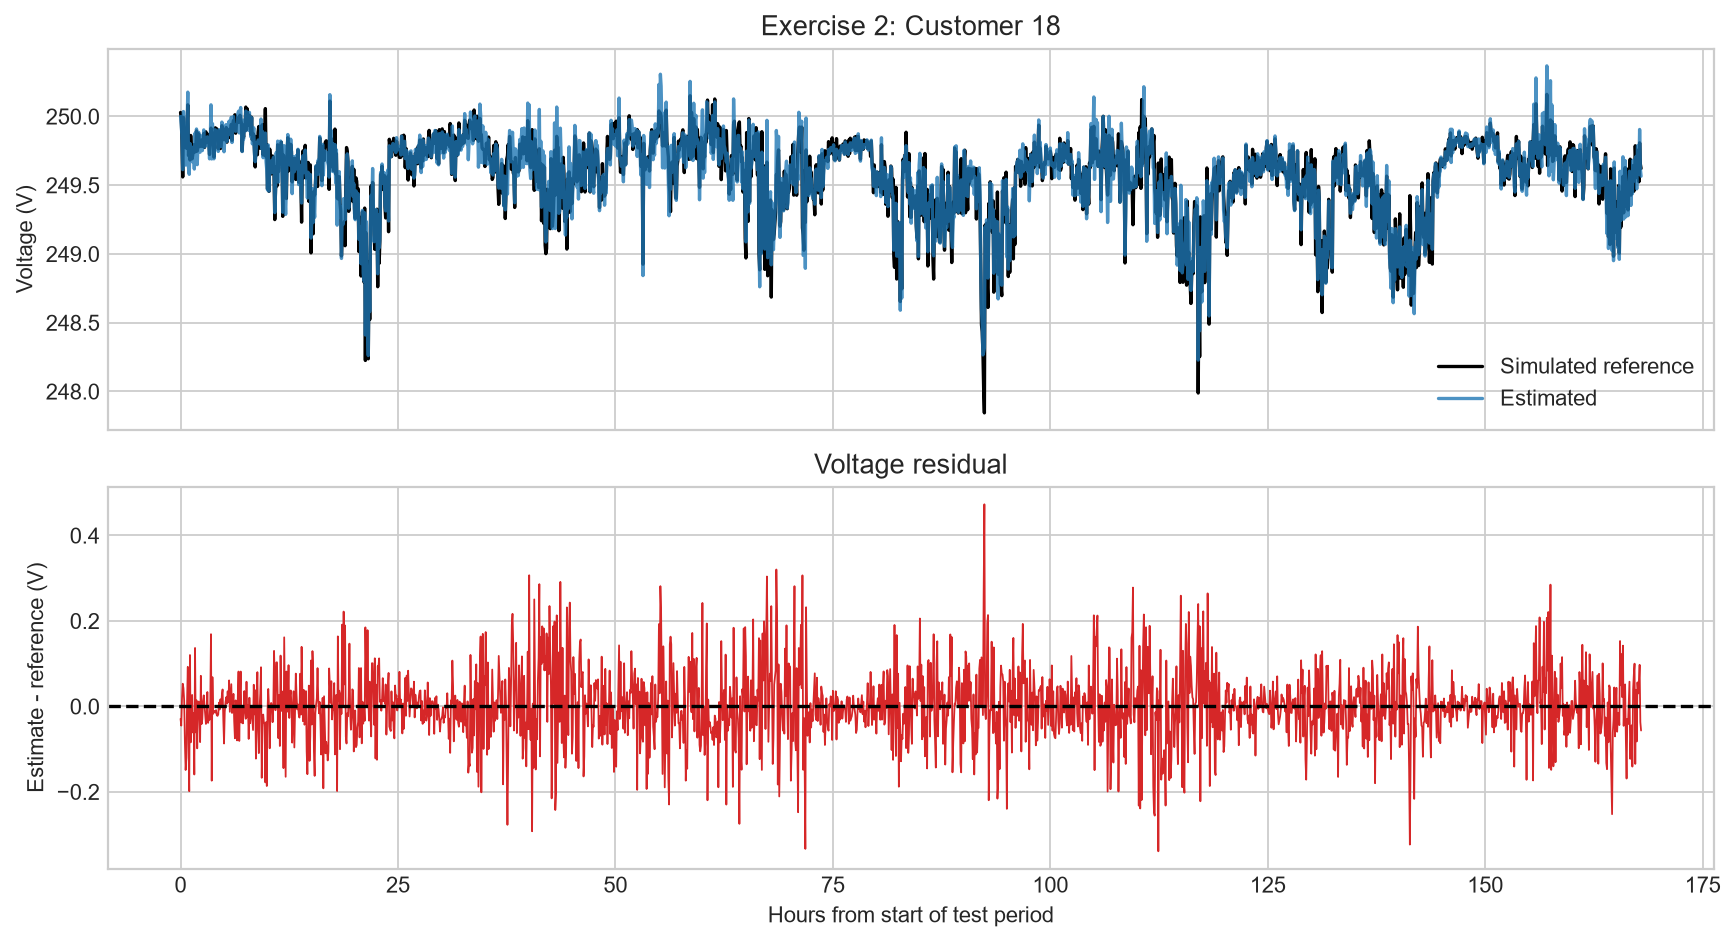
\includegraphics[width=\linewidth]{assets/exercise_voltage_profiles.png}
  \caption{Voltage estimates and residuals for the highest-RMSE customer
  over the full test period, produced by E2.4.}
\end{figure}

\end{document}
